% * * * * * * * * * * * * * * * * * * * * * * * * * * * * * * * * * * *
% *                             Thesis                                *
% *                 https://github.com/Jacopx/Thesis                  *
% * * * * * * * * * * * * * * * * * * * * * * * * * * * * * * * * * * *

\documentclass[%
    corpo=12pt,
    twoside,
%    stile=classica,
    oldstyle,
    autoretitolo,
    greek,
    evenboxes,
%    tipotesi,
]{toptesi}
%%%%%%%%%%%%%%%%%%%%%%%%%%%%%%%%%%%%%%%%%%%%%%%%%%%%

\usepackage[utf8]{inputenc}
\usepackage[T1]{fontenc}
\usepackage{lmodern}
\usepackage{hyperref}
\usepackage{graphicx}
\usepackage{subfigure}
\usepackage{booktabs}
\usepackage{amsfonts}
\usepackage{amsmath}
\usepackage{amssymb}
\usepackage{bm}
\usepackage{listings}

\hypersetup{%
    pdfpagemode={UseOutlines},
    bookmarksopen,
    pdfstartview={FitH},
    colorlinks,
    linkcolor={blue},
    citecolor={blue},
    urlcolor={blue}
  }

%%%%%%% Definizioni locali

\interlinea{1.5} 


\begin{document}

\ateneo{Politecnico di Torino}

\titolo{Predizione di difettosità nello sviluppo software attraverso machine learning}
\sottotitolo{Apprendimento automatico applicato all'ingegneria del software}

%
%%%%%%% Corso degli studi
\corsodilaurea{Ingegneria Informatica}% per la laurea

\renewcommand*\IDlabel{}
%
\candidato{Jacopo \textsc{Nasi} [255320]}

%%%%%%% Relatori o supervisori
\relatore{prof.~Maurizio \textsc{Morisio}}

%%%%%%% Tutore
\tutoreaziendale{dott.\ Davide \textsc{Piagneri}}

\sedutadilaurea{\textsc{Aprile} 2020}


%%%%%%% Logo della sede
\logosede{polito}


\frontespizio
\summary
Ogni giorno migliaia di commit vengono eseguiti, ognugno di loro contiene molte informazioni: file modificati, modifiche, commenti, registri di test e molto altro. Una strutturata e corretta gestione delle piattaforme di concontrollo sorgente permette l'estrazione di dati utili analizzabili utilizzando modelli statistici di intelligenza artificiale.\\
Al fine di poter correttamente utilizzare questi dati sono necessari alcuni step preliminari: la prima fase riguarda l'analisi della struttura dati al fine di permettere l'estrazione di tutte le possibili informazioni, successivamente la pre-elaborazione per rimuovere informazioni di inutili e di disturbo, con i dati puliti è possibile procedere con l'estrazione di dati combinati, come la seniority degli sviluppatori, una lista di parole dei componenti modificati, la versione ed altre informazioni di carattere più matematico. L'ultima fase prevede la sostituzione dell'etichetta testuale relativa alla priorità con un valore numerico corrispondende al valor medio della distribuzione della durata di quella etichetta, questo valore prenderà il nome di severity. I dati verranno poi aggregati per settimana.
Una volta generati i dati verranno utilizzati per allenare tre differenti modelli: Random Forest, Gradient Boosting e Reti Neurali. L'allenamento sarà gestito in tre differenti modalità: la prima allena e predice utilizzando lo stesso filone di dati, la seconda, cross-version, prevede che il modello venga allenato su dati relativi ad alcune versione del progetto per poi effettuare la predizione sulle successive, la terza, cross-project, allena il modello con dati relativi ad un progetto per poi prevedere l'andamento di uno differente.\\
Tutti le tipologie ottengono dei buoni risultati, il migliore è quello cross-project che riesce ad ottenere una precisione maggiore del 90\% fino a quattro settimane e comunque maggiore del 70\% fino a 20 settimane.


\acknowledgements
Un ringraziamento speciale a Smirnuff ed i suoi cavalieri, luce della mia battaglia.

\indici

\mainmatter

% #######################################
% #            Introduction             #
% #######################################

\chapter{Introduzione}
\label{chap:intro}
\section{Problema Generale}
Lo sviluppo software non si presenta molto differente dallo sviluppo di qualsiasi altro prodotto, dopo una fase iniziale di progettazione lo sviluppo del codice può avere inizio, durante esso emergeranno sistematicamente dei problemi che dovranno essere risolti prima della consegna della versione finale.\\
Ogni progetto software è costituito da diversi commit per giorno, ognugno di essi contiene innumerevoli informazioni le quali possono essere utilizzate per analisi statistiche. La predizione della difettosità può migliorare enormemente il processo di sviluppo, allocando un corretto numero di sviluppatori per risolvere le problematiche e riducendo quindi le tempistiche per la correzione. Anche il machine learning può essere utilizzato per la predizione dei difetti.\\
La predizione è uno strumento sempre più utilizzato a livello industriale, un corretto utilizzo può generare enormi benifici a livello produttivo, permettendo la riduzione di sprechi, l'ottimizzazione delle vendite e tante altri vantaggi. Lo sviluppo di progetti di natura informatica è sempre di più centrale all'interno della nostra società attuale, anche questo processo potrebbe trarre beneficio dai vantaggi della predizione. L'implementazione di tecniche statistiche viene in supporto, vista la natura intellettuale della programmazione, nello generazione di predizioni utili.

\section{Strumenti utilizzati}
Lo sviluppo di questo progetto a richiesto l'utilizzo di diversi strumenti, di seguito una lista degli stessi:

\paragraph{\href{https://www.python.org/}{Python}} Il linguaggio di programmazione principale, utilizzato per la gestione dei dati, l'estrazione di informazioni, l'applicazione di algoritmi matematici e l'interazione con altri software. Nello specificio la versione utilizzata è stata la v3.7.0

\paragraph{\href{https://pandas.pydata.org/}{Pandas}} Libreria open source ad alte prestazioni, con semplici strutture e strumenti adatti all'analisi dati attraverso Python.

\paragraph{\href{https://numpy.org/}{NumPy}} Libreria per il calcolo scientifico attraverso Python.

\paragraph{\href{https://matplotlib.org/}{Matplotlib}} Libreria per il disegno di grafici 2D in Python.

\paragraph{\href{https://seaborn.pydata.org/}{Seaborn}} Libreria avanzata per il disegno 2D in Python.

\paragraph{\href{https://www.tensorflow.org/}{Tensorflow}} Piattaforma per machine learning.

\paragraph{\href{https://keras.io/}{Keras}} API di alto livello per reti neurali.

\paragraph{\href{https://scikit-learn.org/stable/}{SciKit-Learn}} Strumenti e librerie per machine learning.

\paragraph{\href{https://gitlab.com}{GitLab}} Piattaforma di sourcing basata su Git. Utilizzata per il codice sorgente del progetto.
% \url{https://gitlab.com/EiS-Projects/analytics/temp/thesisProjectJN}.

\paragraph{\href{https://github.com}{GitHub}} Piattaforma di sourcing basata su Git. Utilizzata per il calendario e elaborato testuale:
\begin{itemize}
  \item Tesi: \url{https://github.com/Jacopx/Thesis}
  \item Calendario: \url{https://github.com/Jacopx/ThesisCalendar}
\end{itemize}

\paragraph{\href{https://www.jetbrains.com/}{JetBrains IDEs}} IDE per lo sviluppo di diversi linguaggi di programmazione, gratuita per gli studenti:
\begin{itemize}
  \item PyCharm: \url{https://www.jetbrains.com/pycharm/}
  \item DataGrip: \url{https://www.jetbrains.com/datagrip/}
\end{itemize}

% #######################################
% #            State of art             #
% #######################################
\chapter{Stato dell'arte}
\section{Lavori correlati}
Parlando di altri lavori su simili tematiche.

% #######################################
% #              Datasets               #
% #######################################

\chapter{Dati}
\label{chap:dataset}
Le seguenti sezioni analizzeranno le basi di dati utilizzate in questo progetto.
\section{SEOSS33}
SEOSS33\cite{SEOSS33} è una \href{https://doi.org/10.7910/DVN/PDDZ4Q}{base dati} collezionante errori, issue e tante altre informazioni a proposito di 33 progetti open source. I dati sono stati tutti collezionati estraendo le informazioni dalle piattaforme di controllo del codice sorgente, Version Control System (VCS), come GitHub e dalle piattaforme per la gestione dello sviluppo, Issue Tracking System (ITS), come Jira di Atlassian.\\
Ad oggi nessun altro progetto di ricerca, su questi dati, è stato effettuato.\\
Ogni progetto prevede una propria linea durante la fase di sviluppo, tutte le metodologie e linee guida sono alla base degli studi di ingegneria del software. Tuttavia è possibile unificare ed accorpare secondo una categorizzazione standar molte delle differenze specifiche. Lo svilluppo della base dati SEOSS33 mira proprio alla creazione di un serie di dati generalizzati e fruibili attraverso medesime procedure senza la necessità di adattarsi alle specifiche caratteristiche di ogni singolo progetto.\\
Il mondo open source presenta una quantità pressochè infinita di differenti software, parte del progetto in questione è stata dedicata alla selezione dei software da analizzare per l'inserimento nella base dati condivisa, per questo motivo sono state definite alcune carattestiche che accomunassero i vari progetti in modo da costituire una base: discretamente omogenea a livello di dimensionalità, ma con differenze struttuali utili per successive analisi come quella relativa a questo progetto. Il requisito principiale riguardava il linguaggio di programmazione, considerare progetti sviluppati per la maggior parte in un singolo linguaggio di programmazione permette di ridurre la variabilità interna ad ogni singolo progetto. Vista la natura di analisi attraverso il machine learning, un'altra importante carattestica riguardava il numero di issue, il quale doveva essere sufficientemente elevato. I progetti, oltre a dover essere attualmente in sviluppo, dovevano presentare un età di almeno 3 anni. La definizione di tutti questi parametri a permesso di generare una base dati contenente 33 progetti simili come struttura ma con caratteristiche differenti.\\
Lo sviluppo del presente progetto di tesi si è concentrato solamente su cinque di questi schemi, sono stati scelti i progetti più grossi e quelli in sviluppo dal maggior tempo, nello specificio i selezionati sono riportati in tabella \ref{tab:seoss33_selected}:
\begin{center}
  \captionof{table}{Distribuzione dati} \label{tab:seoss33_selected}
  \begin{tabular}{ |c|c|c| }
     \hline
     \textbf{Progetto} & \textbf{Mesi} & \textbf{Issue} \\
     \hline
     \hline
     Hadoop & 150 & $39086$ \\
     Hbase & 131 & $19247$ \\
     Maven & 183 & $18025$ \\
     Cassandra & 106 & $13965$ \\
     Hive & 113 & $18025$ \\
     \hline
  \end{tabular}
\end{center}

Al fine di generalizzare le specifiche differenze, le varie issue: \textit{New Feature}, \textit{Bug Report}, ecc... Sono state mappate su cinque categorie:
\begin{itemize}
  \item Bug: Un problema che previene il funzionamento del prodotto
  \item Feature: Una nuova funzionalità del prodotto
  \item Improvement: Un miglioramento di una funzionalità già esistente
  \item Task: Un compito necessario
  \item Other: Vario
\end{itemize}

La figure \ref{fig:prior} visualizza la distribuzione, rispetto le varie categorie, del numero di issue per ogni progetto.

\begin{figure}[!ht]
  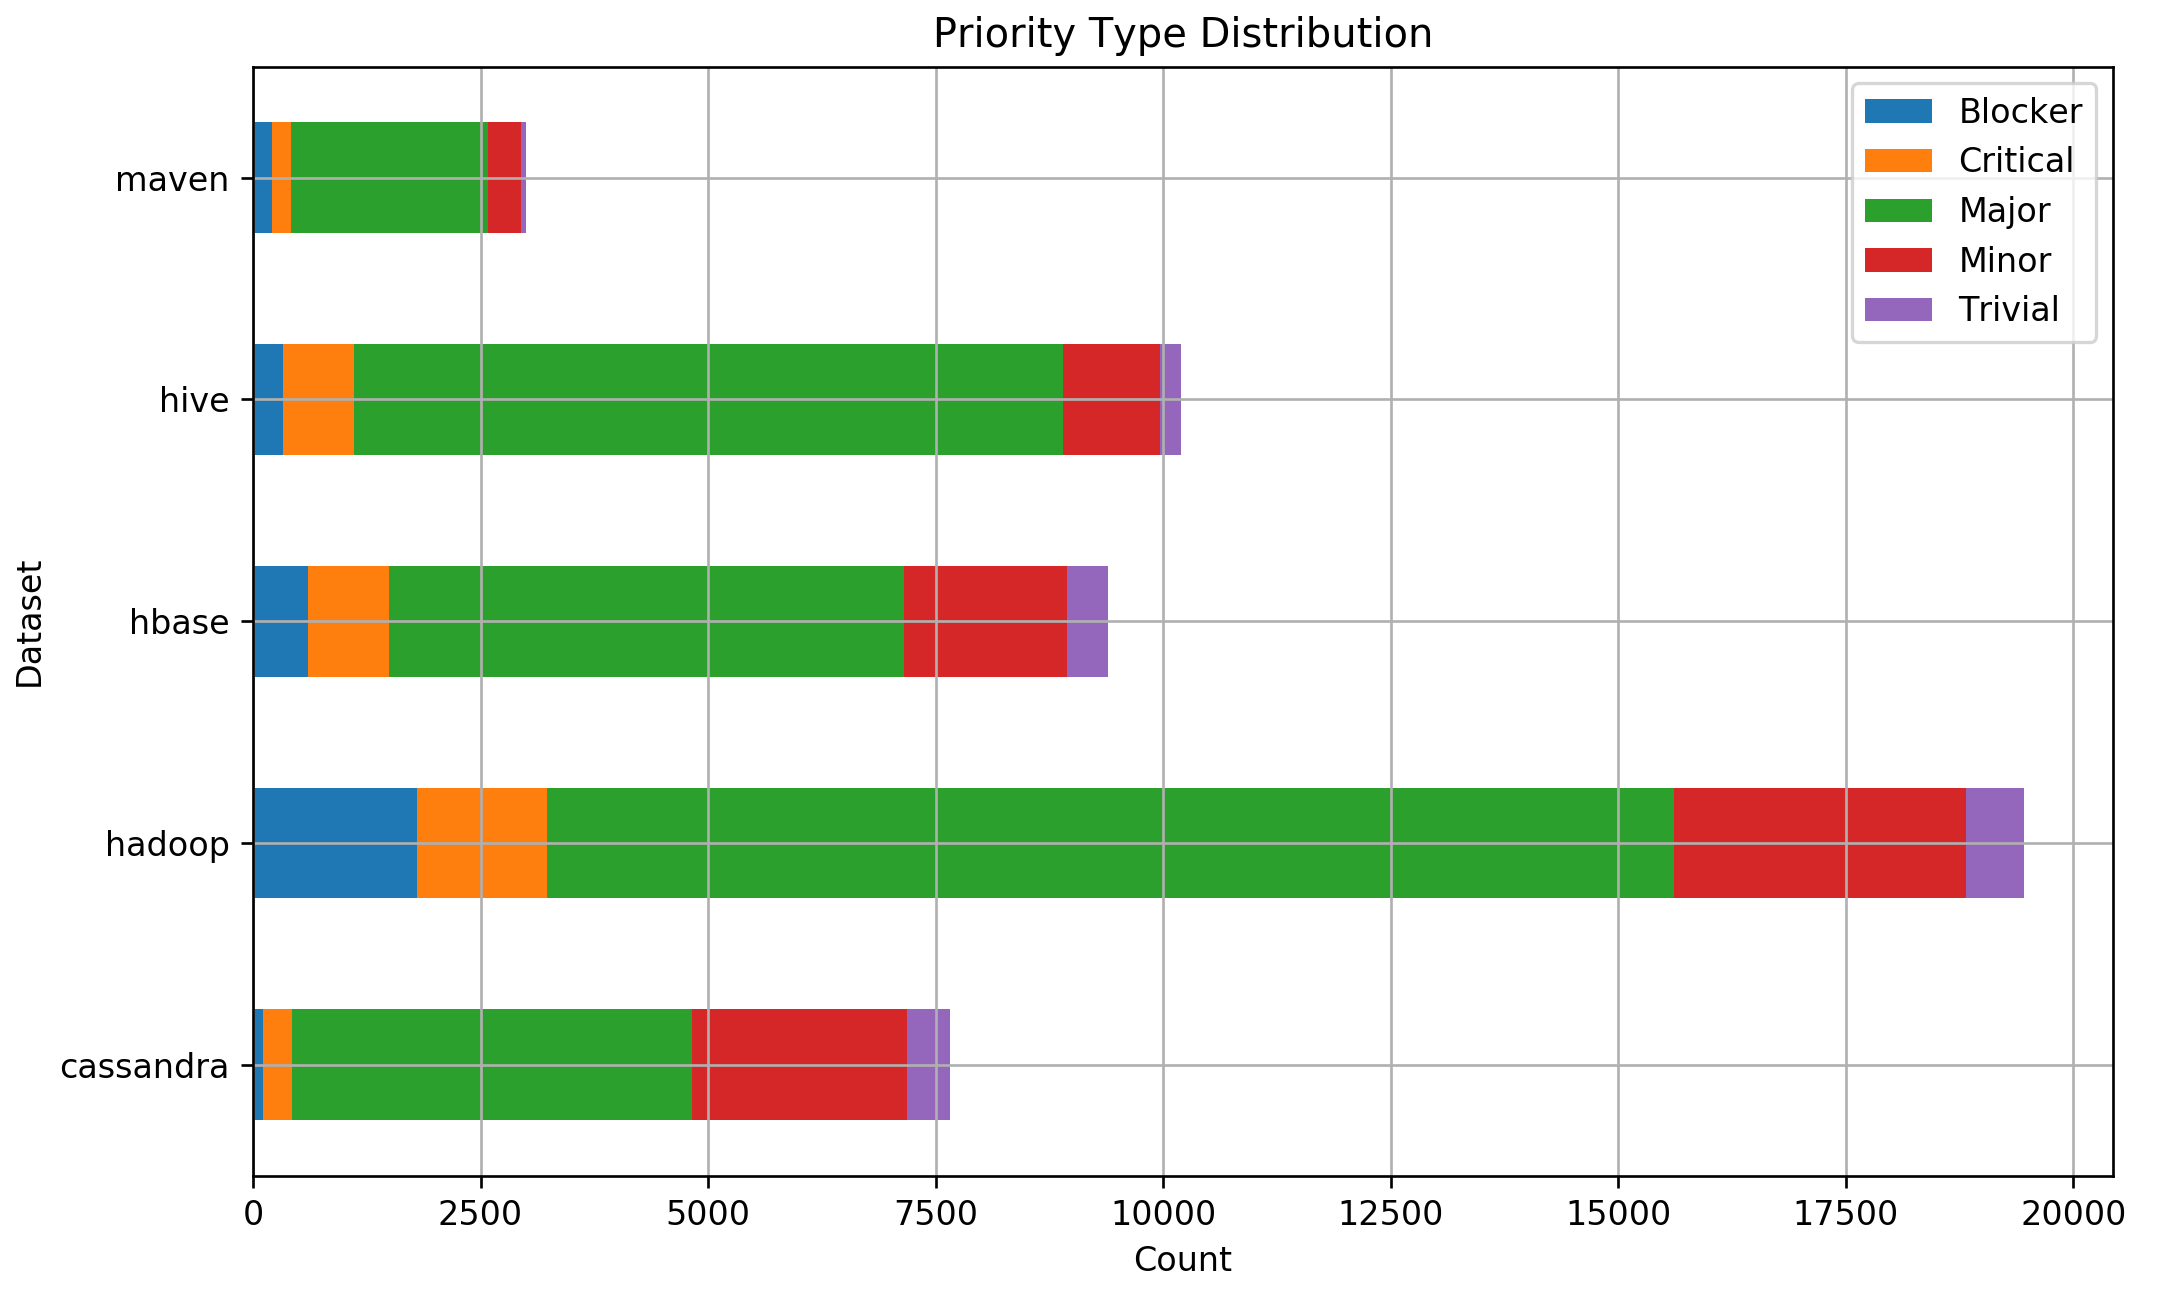
\includegraphics[width=\linewidth]{figure/prior.png}
  \caption{Distribuzione issue per progetto}
  \label{fig:prior}
\end{figure}

Per poter estrarre ed utilizzare al meglio i dati è necessario conoscere al meglio la struttura contenitore.
I dati relativi ad ogni software sono salvati in un file SQLITE, un database SQL offline che permette l'accesso sfruttando le potenzialità delle query, senza la necessità di un server vero e proprio. La figura \ref{fig:seoss33_db} riporta lo schema integrale della struttura.\\
Tutto il modello si basa sulla sua entità centrale, la issue, ovvero l'attività di segnalazione che è stata creata da uno sviluppatore per gestire una problematica. Ognugna di queste issue è caratterizzata dal proprio \textit{issue\_id} il quale ne rappresenta la chiave primaria ed univoca, normalmente è strutturata con il nome del progetto seguito da un numero progressivo. La tabella relativa alle issue contiene ulteriori informazioni direttamente correlate, la tipologia, la priorità, le informazioni temporali di apertura, aggiornamento e chiusura della stessa, un breve riassunto della problematica, lo stato e le informazioni relative allo sviluppatore che l'ha aperta. Direttamentamente collegate, tramite la chiave primaria, vi sono le tabelle contenenti i commenti \textit{issue\_comment}, la versione \textit{issue\_fix\_version}, il componente modificato \textit{issue\_component} ed la tabella \textit{change\_set\_link} la quale collega i vari commit alle issue. Durante l'estrazione delle varie informazioni sono state utilizzate tute le tabelle ad esclusione di \textit{issue\_link} la quale viene utilizzare per correlare le differenti issue tra di loro.

\begin{figure}[!ht]
  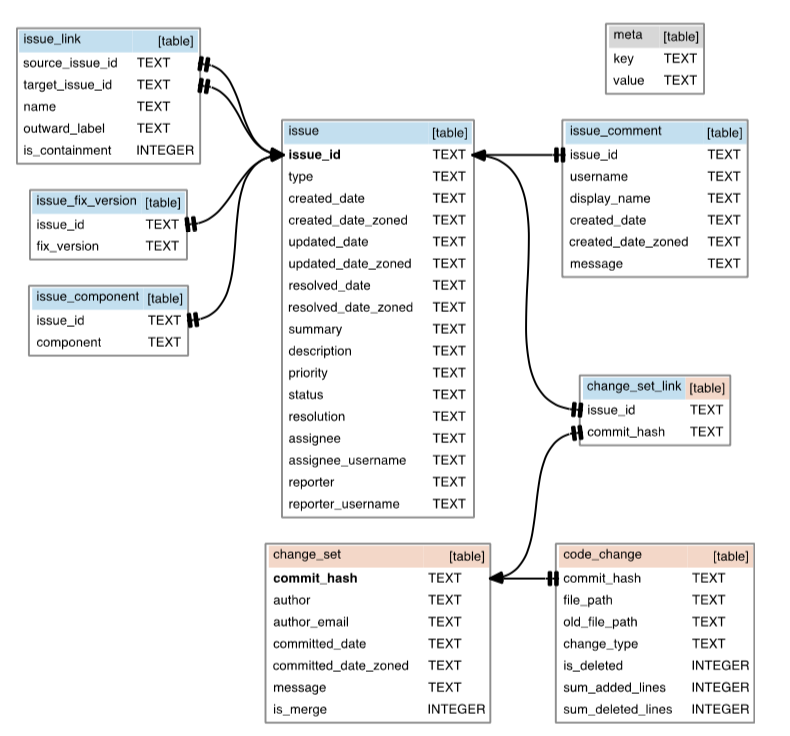
\includegraphics[width=\linewidth]{figure/seoss33_db_schema.png}
  \caption{Struttura dati di SEOSS33}
  \label{fig:seoss33_db}
\end{figure}

% NOTE: Possibile aggiunger parte relativa all'interfacciamento con questo DB. Informazioni di distribuzione temporale.


% #######################################
% #          Machine Learning           #
% #######################################

\chapter{Apprendimento Automatico}
\label{chap:ml}
\section{Introduzione}
L'apprendimento automatico, meglio conosciuto come Machine Learning (ML), è una branca dell'intelligenza artificiale basata sullo studio di algoritmi e modelli statistici utilizzabili dai calcolatori per svolgere determinati compiti senza essere esplicitamente istruiti per farlo. Questa settore è ormai diventato di dominio pubblico, solo negli ultimi decenni l'ultilizzo di queste tecniche è cresciuto enormemente nonostante la maggior parte di esse furono teorizzate già molti anni prima. La motivazione principale di questo ritardo è da ricercare nella natura stesso di queste strategie, la capacità computazione diventa rilevante e fondamentale all'applicazione degli stessi, grazie alla crescita di essa è ora possibile sfruttare questi algorirmi anche nei computer di casa.\\
Tutti gli algoritmi possono essere catalogati in una delle seguenti categorie:
\begin{itemize}
  \item Knowledge-based: Acquisizione e modellazione di leggi conosciute (dalle regole ai fatti)
  \item Learning: Estrazione della conoscenza e delle regole attraverso esempi ed esperienza (dai fatti alle regole)
\end{itemize}
Tutti gli algoritmi in ambito ML fanno parte della seconda categoria. A loro volta questi algoritmi possono essere divisi in tre principali sotto-categorie: apprendimento supervisionato, apprendimento non supervisionato e apprendimento per rinforzo. Nel primo vengono forniti modelli di dati in ingresso e i dati desiderati in uscita e lo scopo è quello di definire una regola che associ i due parametri. Nel modello non superivisionato il modello ha il compito di trovare una struttura ai dati in ingresso, senza che essi siano precedentemente etichettati in alcun modo. L'ultimo invece viene allenato per un compito, senza che gli venga insegnato come fare ma solamente conoscendo il risultato finale delle proprie azioni.\\
Esisto una varietà enorme di modelli di questa tipologia, i successivi paragrafi tratteranno quelli utilizzati in questo progetto.

\paragraph{Apprendimento Supervisionato}
è una tecnica che prevede di processamento dei dati in ingresso con associati i valori desiderati in uscita, lo scopo del modello è quindi quello di sviluppare una correzione matematica tra tutte le informazioni che riceve in ingresso ed i valori desiderati in uscita. Un volta terminata la fase di allenamento il modello potrà essere utilizzato per prevedere il valore di uscita dati i valori in ingresso. Questa metodologia può essere applicata nella risoluzione di problemi di due differenti categorie, quelli della classificazione e quelli della regressione lineare. Lo scopo del primo è quello di assegnare una etichetta ai dati per classificarli in diverse categorie, per esempio le transazioni sane o fraudolente di una banca. L'assegnazione può essere binaria, quindi solo due etichette, o multi-etichetta. La regressione invece ha l'obbiettivo di predirre un valore continuo di uscita, cercare di sviluppare una relazione matematica tra tute le variabili in ingresso, cercando di prevedere, con il miglior livello di approssimazione il valore finale. Nel nostro progetto verranno solo impiegati questi ultimi, la classificazione non verrà ulteriormente trattata.

\section{Apprendimento ensamble}
L'apprendimento di insieme raggruppa unsa serie di tecniche sviluppate al fine di migliorare i risultati dei singoli prendittori. Invece che utilizzare un singolo modello, nella fase di apprendimento, vengono simultaneamente allenate diverse copie dello stesso modelo con parametri differenti, ciò porterà ad una differenziazione delle risultato di previsione. L'aggregazione, attraverso techinche come bagging, boosting o stacking, permetterà di produrre un risultato più accurato e meno dipendente dalla rumorosità dei dati.

\paragraph{Foresta casuale}
conosciuta anche come Random Forest (RF) è un algoritmo di apprendimento supervisionato, basato sulle metodologie d'insieme, per la classificazione e la regressione. È costituito combinando la predizione di diversi alberi, ognungno allenato separatamente, tramite media \cite{RF_theory}. In figura \ref{fig:rf} una visualizzazione del modello.

\begin{figure}[!ht]
  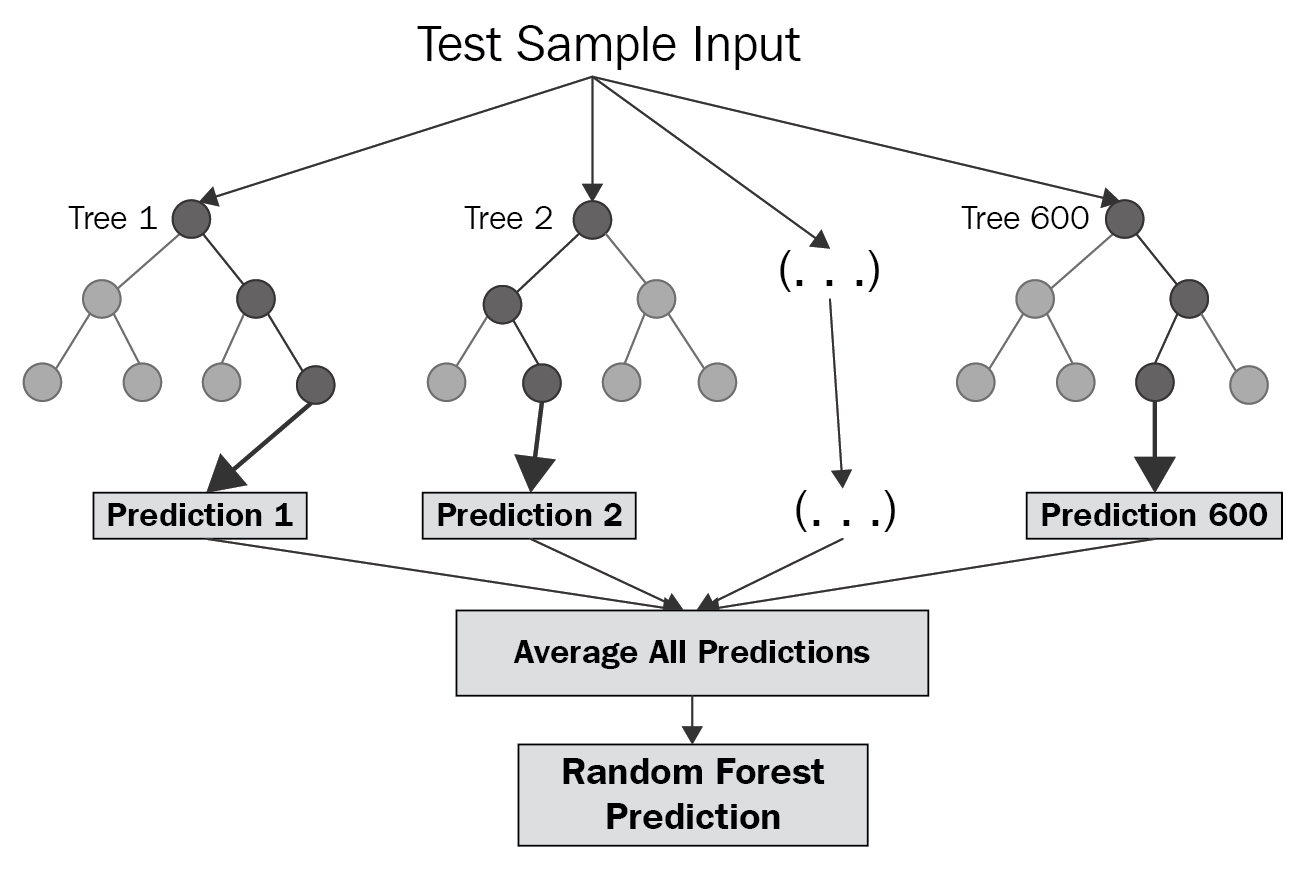
\includegraphics[width=\linewidth]{figure/rf.png}
  \caption{Schema semplificato di foresta casuale \cite{rf}}
  \label{fig:rf}
\end{figure}

La definzione di una foresta richiede tre parametri principali: (1) la metodologia per la divisione in foglie, (2) il tipo di predittore da usare in ciascuna foglia e (3) il metodo per garantire la randomicità.
La divisione in foglia richiede la selezione della forma e metodologia per la valutazione di ogni candidato. Una tipica scelta è quella chiamata axis-aligned, dove i dati vengono diretti nei vari sotto alberi in base al passaggio o meno di un valore soglia, il quale viene scelto casualmente o dalla funzione di ottimizzazione della foglia. Al fine di dividere una foglia vengono generati diversi candidati e viene definito un criterio per scegliere tra essi. Un primo approccio potrebbe essere quello della selezione causuale uniforme, altrimenti la scelta può essere guidata da una funzione di purezza, cercandone la massimizzazione.\\
Possono essere utilizzate diverse techniche per generare casualità nella foresta, attraverso la definizione di soglie senza l'utilizzo di funzioni oppure effettuando con l'allenamento di ogni albero su una selezione di dati ristretta in modo da diversificare direttamente il risultato a livello di insieme.\\
La fase di training viene gestita indipendentemente da ogni alberto attraverso punteggi di struttura e stima, i primi permettono la variazione della forma dello stesso, mentre i secondi guidano le funzioni di ottimizzazione delle singole foglie.\\
Un volta effettuato l'allenamento della rete è possibile utilizzare il modello per la predizione dei valori. Nella fase di stima, ogni singolo albero, generera indipendemente un proprio valore, la scelta finale avverrà calcolando la media aritmetica di tutti questi valori generati, il contributo è equamente ripartito tra tutti.\\
La nostra implementazione sfrutta le API per la Random Forest di SciKit-Learn v0.21:
\begin{lstlisting}[language=python, frame=single]
  from sklearn.ensemble import RandomForestRegressor
\end{lstlisting}
Gli specifici parametri utilizzati verranno illustrati durante il capitolo \ref{chap:forecasting} sulla predizione.

\paragraph{Macchine ad aumento di gradiente}
conosciute anche come Gradient Boosting Machines (GBM), sono una famiglia di potenti modelli statistici di apprendimento automatico in grado di ottenere ottimi risultati in una grande varietà di applicazioni. Una delle loro principali caratteristiche è la possibilità di personalizzare il modello in base alle caratteristiche dell'applicazione \cite{gbm}. Tecniche come la foresta casuale, appena trattata, sono basate sulla semplice media dei risultati prodotti da ogni singolo componente. La famiglia dei metodi di aumento è basata su una differente strategia di unione dei pezzi per la formazione della modello finale. Il boosting aggiunge, sequenziamente, nuovi parti all'insieme; durante la fase di allenamento vengono via via sviluppati nuovi piccoli modelli da aggiungere al fine di migliorare l'accuratezza nella previsione. Idealmente vengono costruiti nuovi modelli di base, come per esempio l'albero decisionale, per poter massimizzare la correlazione con il gradiente negativo della funzione di perdita (\textit{loss}).\\
Vista l'alta flessibilità del modello, l'adattamento dello stesso a differenti ambienti non risulta difficoltoso, molte differenti sperimentazioni possono essere fatte.\\
Nel nostro progetto si è deciso di implementare il modello di Gradient Boosting Decision Tree (GBDT) sempre utilizzando la libreria SciKit-Learn v0.21:
\begin{lstlisting}[language=Python, frame=single]
  from sklearn.ensemble import GradientBoostingRegressor
\end{lstlisting}


\section{Reti Neurali}
Le reti neurali, in inglese Neural Networks (NN), sono modelli di apprendimento automatico con diretta ispirazione al cervello umano e come esso procede alla fase di apprensione di un concetto, la rete è costituita dala basilare unità di calcolo, il neurone (neuron), collegata ad altri neuroni attraverso le sinapsi (synapses). La conoscenza è data alla rete, enlla fare di allenamento, attraverso esempi, la forza delle connessione inter neurali è la base per acquisire e mantenere al conoscenza.\\
La fase di apprendimento può essere sia supervisionata che non supervisionata. La modalità supervisionata viene utilizzata per il riconoscimento di schemi (pattern recognition) e regressione e viene effettuata sempre con i dati di input ed i desiderati dati di output. Invece, la modalità non supervisionata, è maggiormente utilizzata per sviluppare modelli adatti al raggruppamento (clustering) e l'allenamento viene effettuato senza il valore desiderato. Il nostro progetto farò uso di reti neurali per la regressione.\\
Questa tipologia di reti può essere di tre tipologie:
\begin{itemize}
  \item Singolo livello flusso in avanti
  \item Multi livello flusso in avanti
  \item Ricorsiva
\end{itemize}
L'architettura standard è composta di tre diversi livelli, figura \ref{fig:mlff}, lo strato di ingresso, le unità nascoste e il livello di uscita; tutti questi livelli sono correlati tra loro tramite le connessioni sviluppate durante la fase di apprendimento.
\begin{figure}[!ht]
  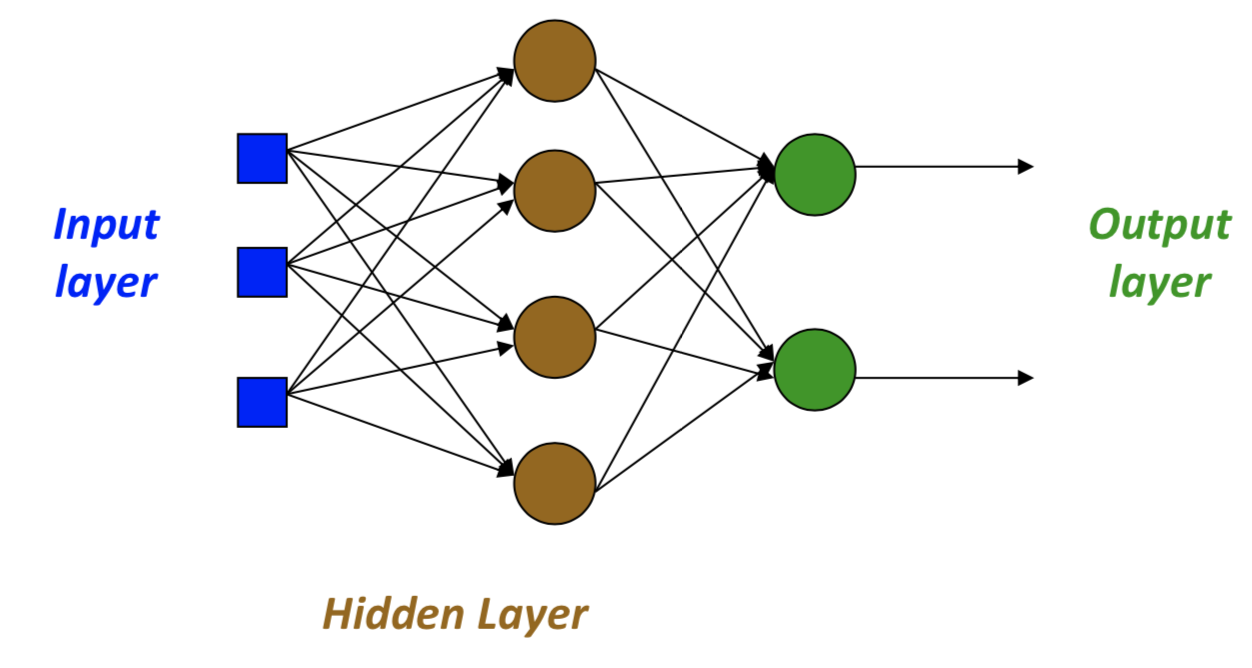
\includegraphics[width=\linewidth]{figure/feed_foward.png}
  \caption{Rete a flusso avanti multi livello}
  \label{fig:mlff}
\end{figure}
Il neurone è l'unità basilare per il processamento all'interno della rete, si occupa di riceve i dati in ingresso, gestirli e poi passarli ai successivi livelli. Ogni ingresso combina i dati con il proprio stato interno e la funzione di attivazione per poi procedere a passare il valore come ingresso del livello successivo. L'importanta che ognugno di questi valori in ingresso avrà sarà determinata dal peso assegnato alla connessione durante la fase di allenamento della rete stessa. Ogni nodo ha la possibilità di ricevere più in un ingresso, per questo motivo, tutti i valori verranno aggregati in modo da consegnare un solo valore come ingresso del successivo strato, la formula per il calcolo della somma è:
\begin{center}
  \begin{equation}
    u = \sum^{m}_{j=1} w_{j}x_{j}
  \end{equation}
\end{center}
Il valore calcolato viene scalato tramite una functione di attivazione $\varphi$ al fine di limitarne l'ampiezza:
\begin{center}
  \begin{equation}
    y = \varphi(u + b)
  \end{equation}
\end{center}
La precedente funzione riporta il parametro $b$ il quale rappresenta il bias, un parametro esterno del neurone. $y$ rappresenta invece il valore di uscita dopo la computazione, il quale rappresenta il valore di ingresso del successivo livello gerarchico. Un esempio della struttura in questione si può trovare in figura \ref{fig:neuron}.
\begin{figure}[!ht]
  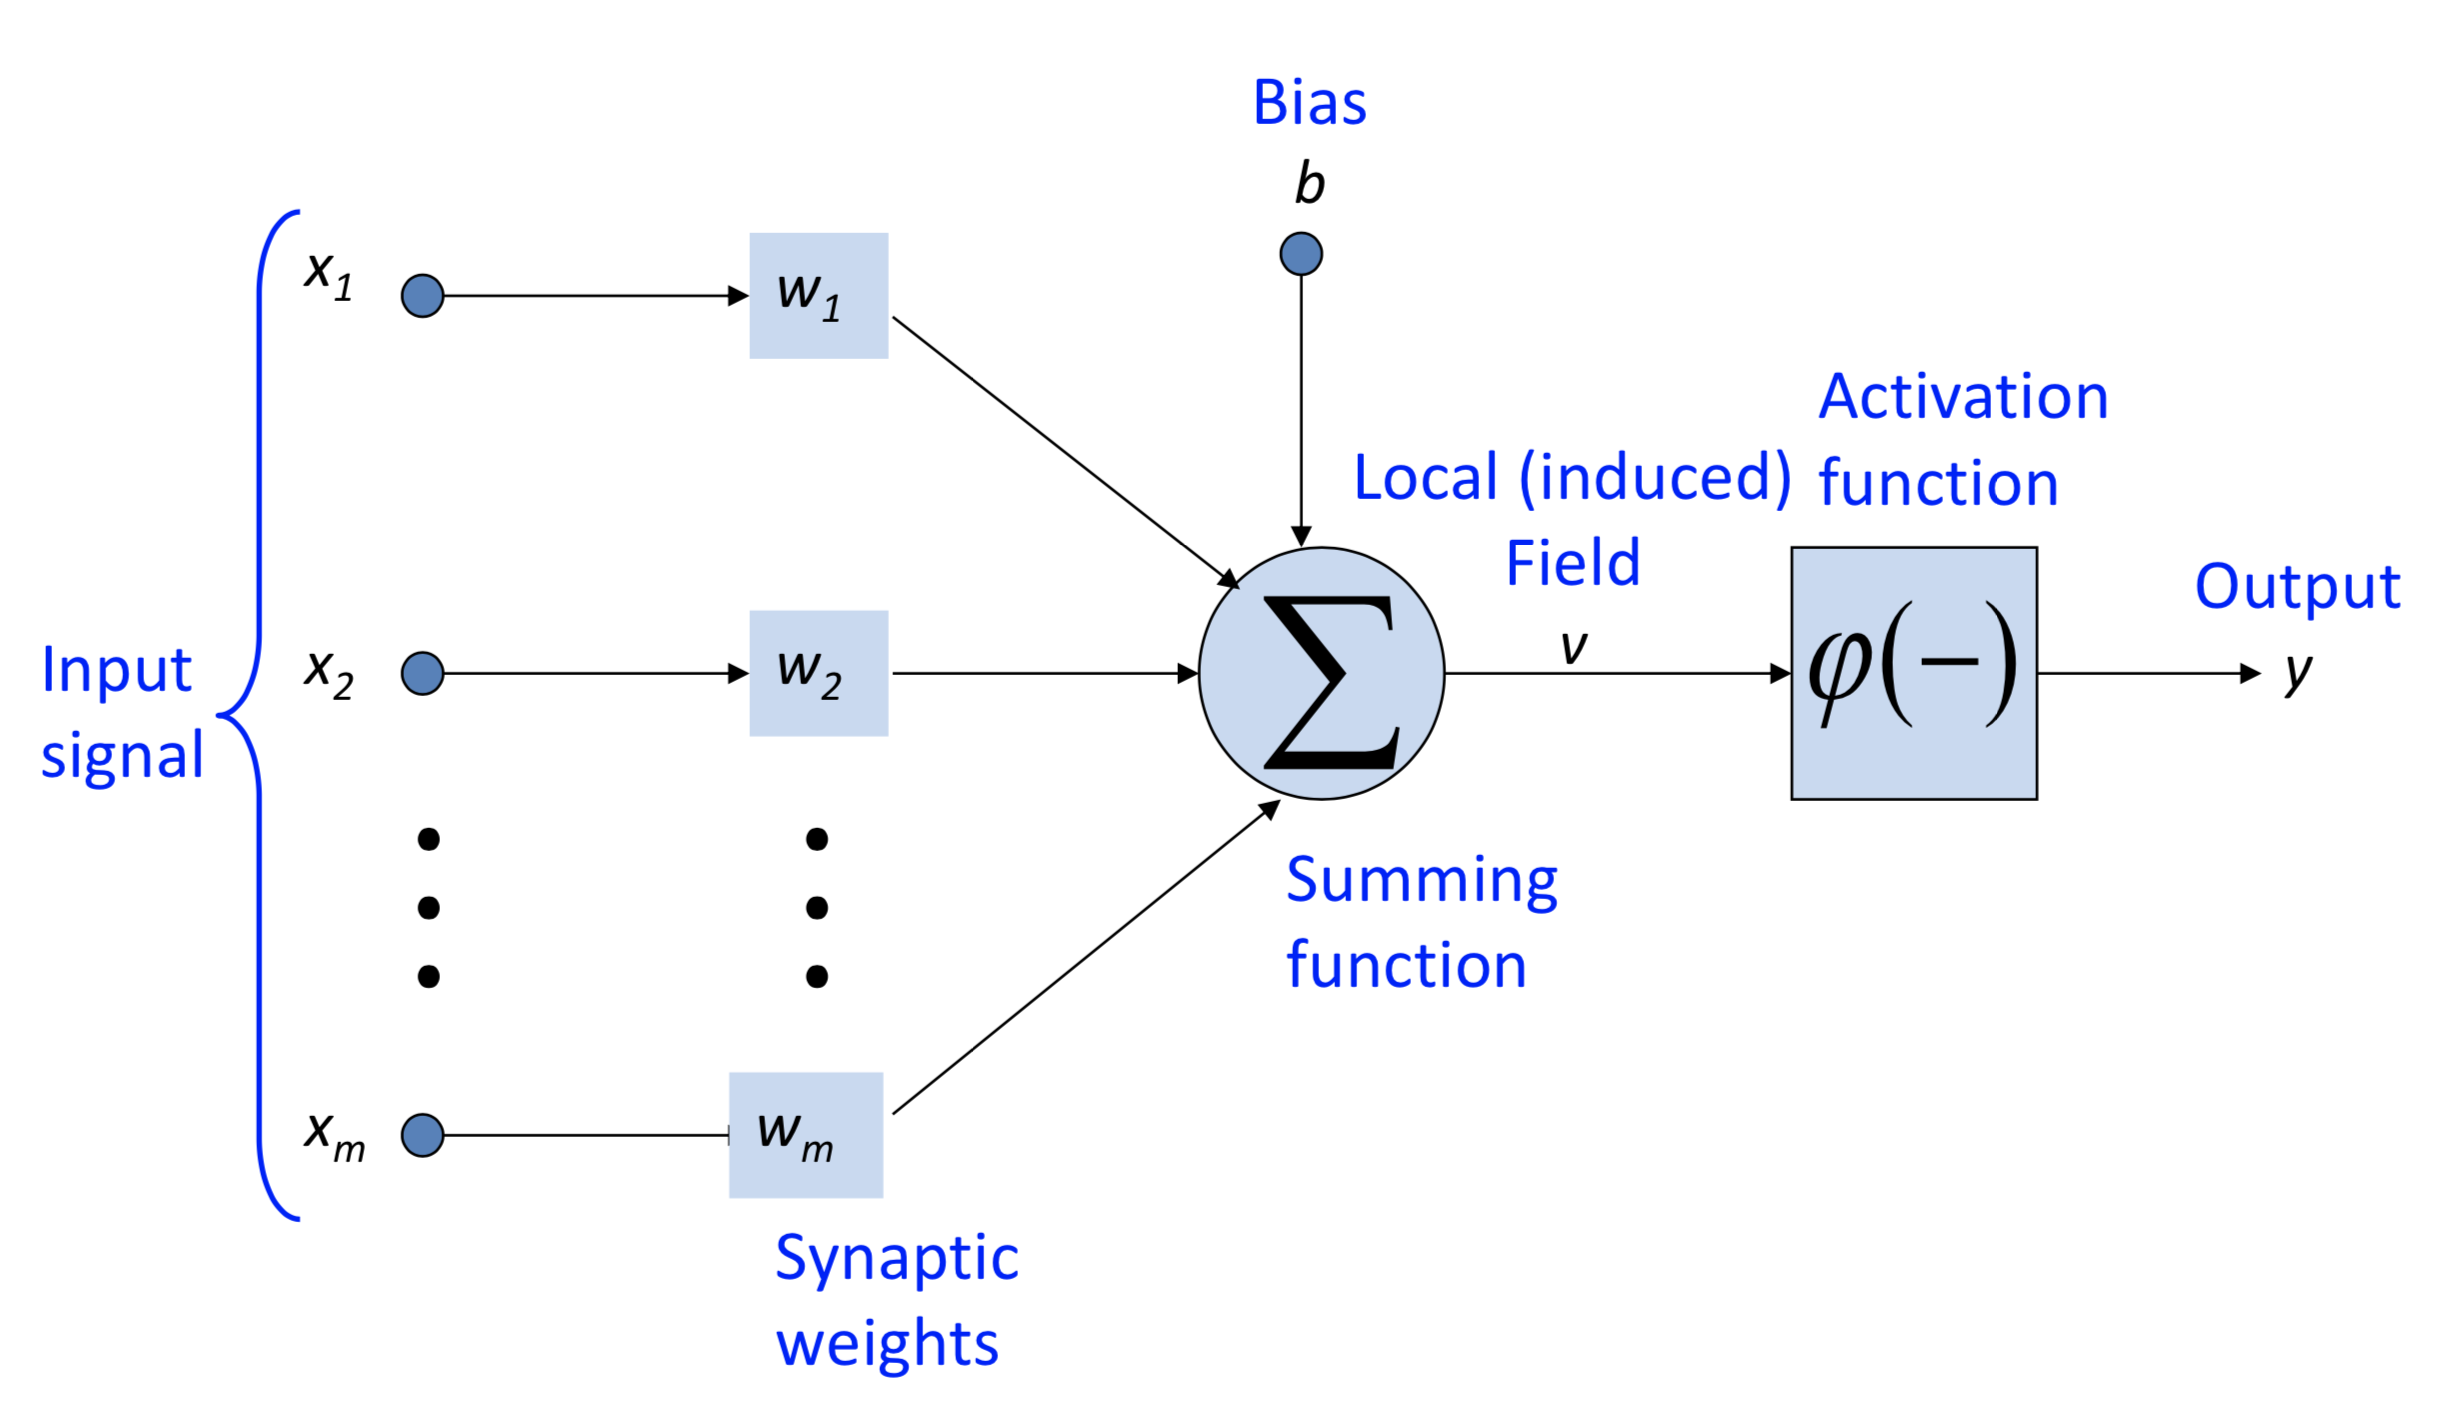
\includegraphics[width=\linewidth]{figure/neuron.png}
  \caption{Visualizzazione di neurone}
  \label{fig:neuron}
\end{figure}

Diverse funzioni di attivazione possono essere applicate al neurone, il loro compito è quello di emulare la tipica risposta biologica del sistema nervoso umano e le sue differenti metodologie di attivazione. Nel corso degli anni sono state definite numerose differenti funzioni, più o meno adatte a differenti contesti, con proprie peculiarità, problematiche e carattestiche. Possono essere classificate in due categorie, lineari e non lineari, le più comuni sono: lineare, gradino, relu e sigmoide.

\paragraph{Gradino} è una delle più comuni funzioni di attivazione, binaria, lineare e basata su soglia, in figura \ref{fig:step} la sua definizione. Quando il valore in ingresso è sopra o sotto la soglia definita, il neurone viene attivano e passa il valore in ingresso al successivo livello. La principale problematica correlata a questa funzione è la sua impossibilità di gestire valori multipli in uscita.

\paragraph{Lineare} è una funzione di attivazione lineare della forma:
\begin{center}
  \begin{equation}
    f(x) = x
  \end{equation}
\end{center}
La funzione, dato il valore in ingresso e moltiplicandolo per il peso del neurone, calcola il valore di uscita. Rispetto alla funzione gradito possono essere generati output multi valore, presenta comunque due problematiche: non sarà possibile utilizzare la retropropagazione (trattata successivamente) per allenare la rete, vista la funzione derivata costante; l'altro problema riguarda il collasso di tutto i diversi livelli in uno solo, vista la sua natura lineare, il valore di uscita finale sarà in ogni caso la combinazione lineare tutti i livelli precedenti. La figura \ref{fig:linear} visualizza la curva in questione.

\begin{figure}
  \centering
  \begin{minipage}{.5\textwidth}
    \centering
    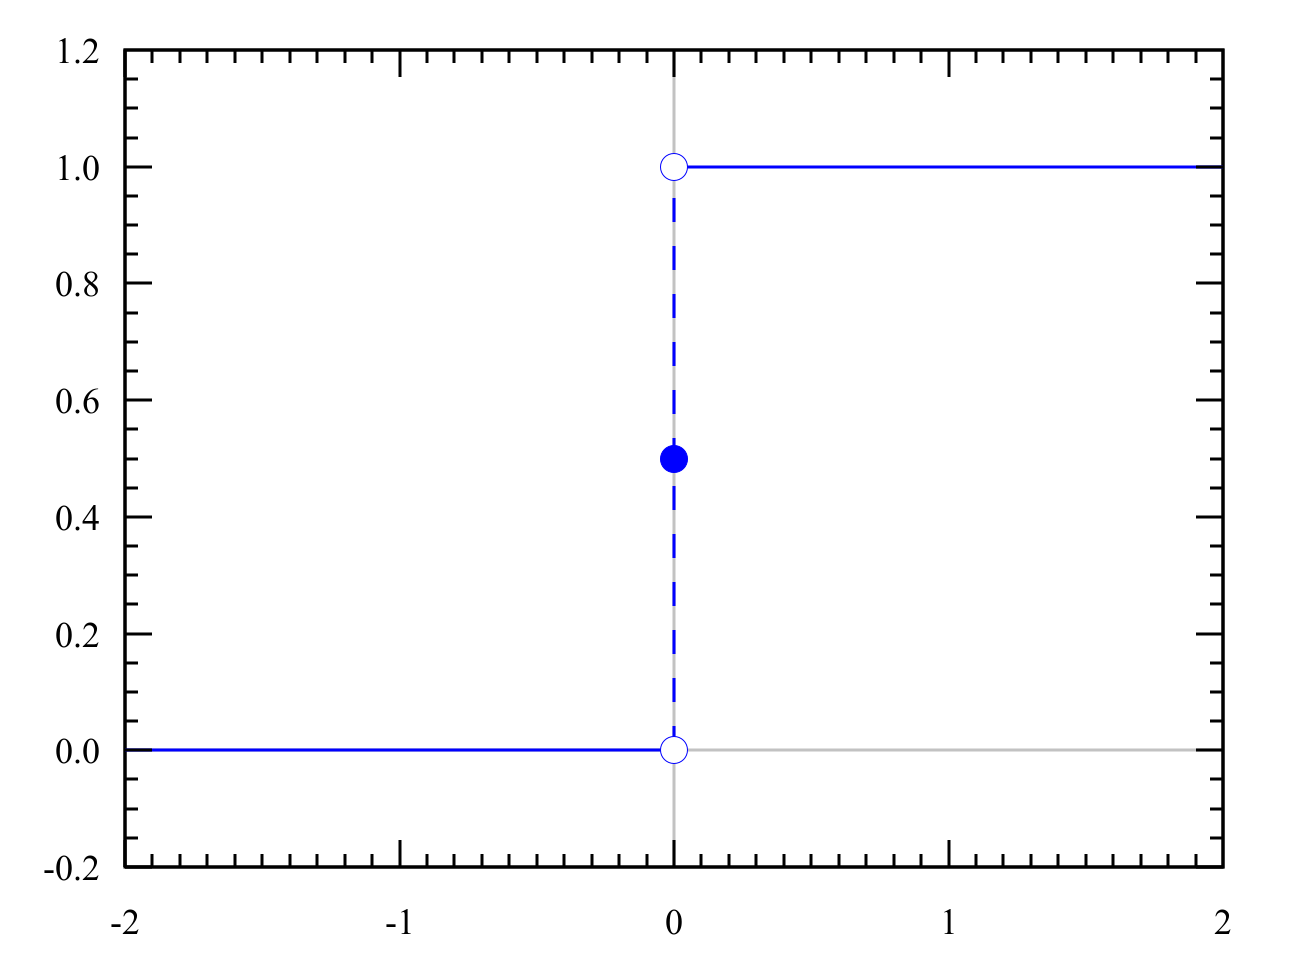
\includegraphics[width=0.85\linewidth]{figure/step.png}
    \caption{Funzione a gradino}
    \label{fig:step}
  \end{minipage}%
  \begin{minipage}{.5\textwidth}
    \centering
    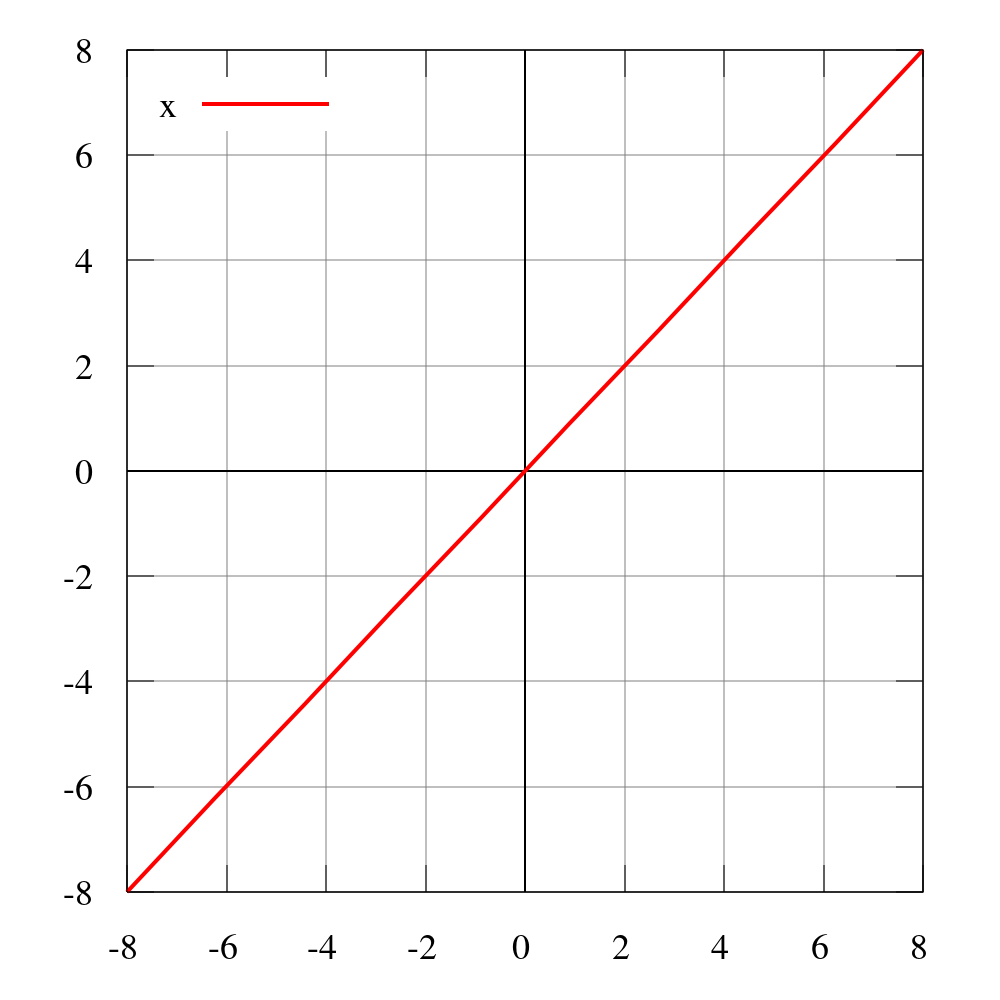
\includegraphics[width=0.75\linewidth]{figure/linear.png}
    \caption{Funzione lineare}
    \label{fig:linear}
  \end{minipage}
\end{figure}

\paragraph{Sigmoide} è la prima funzione di attivazione non lineare trattata, nello specifico è caratterizzata dalla seguente equazione:
\begin{center}
  \begin{equation}
    f(x) = \frac{1}{1+e^{x}}
  \end{equation}
\end{center}
La peculiare caratteristica di non linearità permette un più morbido gradiente in modo da prevenire valori vuori scala, normalizzando il valore tra $[0, +1]$ si ottengono anche benifici a livello di pulizia dei dati in ingresso utilizzati successivamente per le previsioni. La funzione non si presenta esente da problematiche, la principale riguarda la vanificazione del gradiente, se da un lato permette di smorzare i valori fuori scala, si tramuta in collo di bottiglia in altri casi, in caso di valori in ingresso molto elevati o molto bassi non vi sarà differenziazione nel valore di uscita. Inoltre l'applicazione del calcolo stesso è decisamente più impegnativa a livello computazione. La figure \ref{fig:sigmoid} descrive la curva in questione.

\paragraph{ReLU} il quale acronimo sta per Rectified Linear Unit, unità lineare rettificata, è definita nella seguente maniera:
\begin{center}
  \begin{equation}
    f(x)= max(0, x)
  \end{equation}
\end{center}
Nonostante assomigli molto alla funzione di attivazione lineare, presenta una funzione derivate che permette la retropropagazione e si presenta molto efficiente a livello computazione. Le problematiche si presentano in caso di valori in ingresso prossimi allo zero o addirittura negativi, il gradiente della funzione diventa nullo e la rete non potra effettuare la retropropagazione e conseguentemente non potrà portare avanti il processo di apprendimento.

\begin{figure}
  \centering
  \begin{minipage}{.5\textwidth}
    \centering
    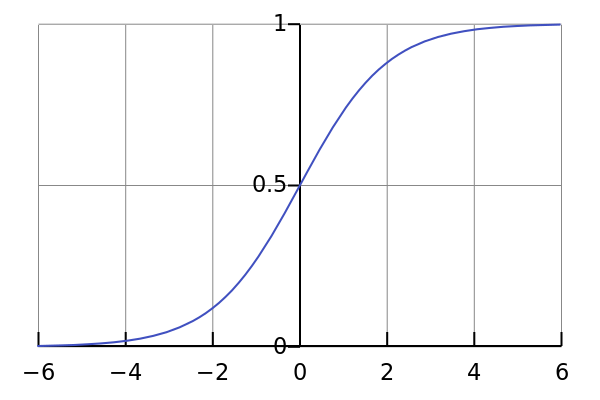
\includegraphics[width=0.8\linewidth]{figure/sigmoid.png}
    \caption{Sigmoide}
    \label{fig:sigmoid}
  \end{minipage}%
  \begin{minipage}{.5\textwidth}
    \centering
    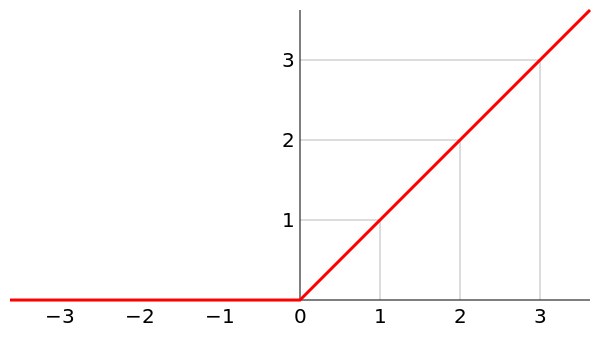
\includegraphics[width=0.8\linewidth]{figure/relu.png}
    \caption{ReLU}
    \label{fig:relu}
  \end{minipage}
\end{figure}

\paragraph{Regola di apprendimento delta} è basata sulla differenza tra il valore in uscita di riferimento e quello ottenuto dal modello e viene utilizzata per guidare la fase di apprendimento del modello stesso. Ogni volta che il valore in uscita viene calcolato il valore the peso del neurone viene corretto basandosi su una funzione di errore con l'obbiettivo di ridurre la differenza tra i due valori in esame. 

\paragraph{Retropropagazione dell'errore} conosciuta in inglese come backpropagation, è un algortimo per l'apprendimento supervisionato delle reti neurali artificiali basando sul gradiente discendente. Data una rete neurale ed una funzione di errore, il metodo calcola il gradiente della funzione riguardante i pesi della rete. È una generalizzazione della regola delta per i percetroni di reti multi livello a flusso avanti \cite{bp}.\\
La principale caratteristica di questa technica è che il gradiente procede all'indietro attraverso la rete, con il gradiente del livello finale calcolato prima di quello del primo livello. Questa soluzione permette un calcolo efficiente del gradiente per ciascuno dei differenti strati. L'algoritmo è strutturato nella seguente maniera:
\begin{enumerate}
  \item Calcolo errore per le unità di uscita
  \item Dal livello ppiù profondo, finchè il primo livello non viene raggiunto:
  \begin{enumerate}
    \item Propagazione dell'errore al precedente livello
    \item Aggiornamento dei pesi tra i due livelli
  \end{enumerate}
\end{enumerate}
La retropropagazione soffre del problema della vanificazione del gradiente, maggiore è il numero di livelli incorporati della rete maggiore sarà la difficoltà per l'allenamento della stessa. Per via della natura della retropropagazione, quando il valore in uscita viene generato, il peso dei neuroni viene aggiornato in accordo alla regola, mano a mano che l'algoritmo procede indietro il potere correttivo diminuisce, il relazione alla derivata della funzione di attivazione; in caso di reti superficiali il problema non si rivela così determinante, il processo avviene senza limitarne gli effetti. In caso di reti più profonde la problematica potrebbe diventare determinante. Una delle possibili soluzioni a questa problematica è l'impiego di funzioni di attivazione adatte, come la ReLU, la quale permette di alleggerire la problematica. Ulteriore soluzione è rappresentata dalla normalizzazione dei dati in ingresso, riscalando opportunamente i dati in entrata tra $[-1, 1]$ è possibile migliorare l'efficacia della procedura, questo perchè i dati verranno tenuti più lontani dagli estremi della funzione di attivazione. Esiste inoltre una tipologia di rete, memorie a lungo-corto termine, in inglese Long Short Term Memory (LSTM), sviluppata appositamente per mitigare il problema della vanificazione del gradiente nelle reti più profonde.

\paragraph{Reti neurali ricorsive} sono una classe di reti neurali che mantiene una connessione tra nodi e sequenze temporali. La principale differenza, rispetto le classiche reti neurali, sono connessioni di feedback, le quali permettono di mantenere traccia di dinamiche temporali. Questa tipologia di reti può processare singoli punti o intere sequenze di dati, come video e discorsi verbali, fondamentale la possibilità per gli step intermedi di mantenere informazioni di input precedenti senza definirne il numero a priori.\\
Questo tipo di strutture viene sfruttato per numerose applicazioni: classificazione di immagini, analisi sentimentale, traduzione macchina, classificazione video, ecc\dots

\paragraph{Memorie a lungo corto termine} le normali reti neurali possono correlare eventi a breve termine con il presente, in alcuni casi può essere sufficiente, in alcuni contesti invece può essere necessaria una connessione con margini più ampi, questo tipo di problematica viene tranquillamente gestito da questo tipo di reti. Cercando di effettuare una previsione sull'ultima parola di una frase tipo: "Il sole splende alto in \textit{cielo}" le parole precedenti all'ultima possono essere sufficienti a determinare un corretto suggerimento da parte della rete. In caso di frasi più complesse potrebbe essere necessaria una maggiore quantità di informazioni, per la frase: "Sono nato in Italia e parlo \textit{italiano}" il contesto si rivela fondamentale al fine di risolvere correttamente la problematica. In questa tipologia di situazione le reti LSTM possono essere di grande supporto.\\
Le reti a memorie a lungo e corto termine sono una tipologia speciale di reti ricorsive, introdotte da Hochreiter \& Schmidhuber (1997) \cite{lstm}, si sono rivelate sempre più utili in ambito previsionale, per la ricerca di schemi ricorrenti a livello temporale. Sono in grado di lavorare su una grandissima varietà di problemi differenti. Normalmente le reti ricorsive si prensentano su un singolo livello, in questo caso la struttura è più complessa ed è costituita da quattro diversi livelli, come visualizzato in figura \ref{fig:lstm}.

\begin{figure}[!ht]
  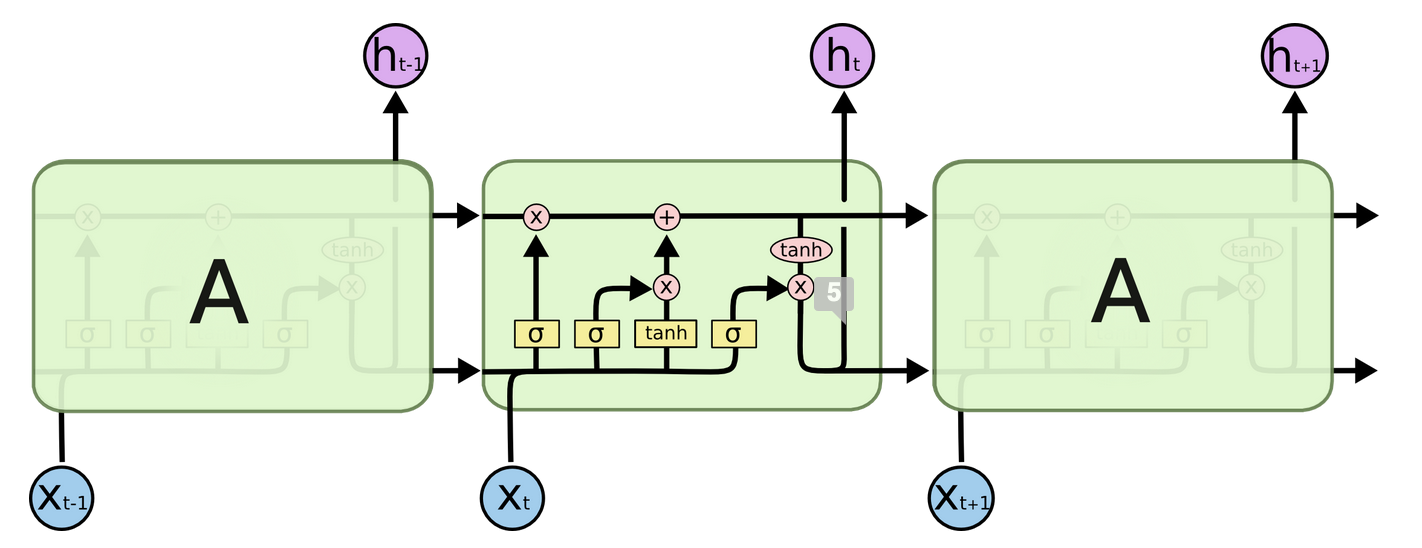
\includegraphics[width=\linewidth]{figure/lstm.png}
  \caption{Struttura rete LSTM \cite{lstm_image}}
  \label{fig:lstm}
\end{figure}

Il primo livello della rete ha il compito di filtrare i dati in input e selezionare cosa mantenere o meno, il secondo passaggio gestirà quali informazioni mantenere nello stato della cella. Il terzo livello invece ha il compito di aggiornare lo stato del nodo in base agli step precedenti. Lultimo livello si occupa invece della scelta del valore di uscita.

\section{Metriche di valutazione}
Ogni modello sviluppato necessità di essere valutato, ci sono innumerevoli modalità per valutare la bontà di un modello, ognuna con proprie caratteristiche. Ovviamente il parere più oggettivo si ottiene sfruttando espressione matematiche, sfortunatamente quest'ultime non sempre sono di facile e rapida comprensione da parte del l'uomo, alcuni errori come quello assoluto, quello relativo possono essere facilmente letti ed interpretati senza alcun tipo di problema; metriche come R2 o l'errore quadratico richiedono una valutazione più approfondita. Dopo attente valutazioni sono state definite alcune metriche che verranno utilizzate nella valutazione dei modelli, di seguito una breve trattazione matematica degli stessi.\\
La maggior parte degli errori deriva dal calcolo di errori più semplici, l'errore assoluto viene calcolato computanto la differenza tra l'obbiettivo $y$ ed il risultato ottenuto $x$:
\begin{center}
  \begin{equation}
    \epsilon = |y - x|
  \end{equation}
\end{center}
Oltre ad essere uno dei più semplici da calcolare risulta anche uno dei più semplici da comprendere in quanto permette di visualizzare direttamente lo scostamento rispetto al valore desiderato.\\
Una prima metrica derivata dall'errore assoluto è l'errore relativo, calcolato dividendo l'errore assoluto per il valore desiderato:
\begin{center}
  \begin{equation}
    \eta = \frac{\epsilon}{|x|} = \frac{|y - x|}{|x|}
  \end{equation}
\end{center}
Questo calcolo riscala direttamente il risultato tra [0, 1], ciò permette una migliore comprensione della differenza. Per esempio, con un valore desiderato di 530 ed un valore stimato di 570 i due errori vengono calcolati come segue:
\begin{center}
  \begin{equation}
      \epsilon = |520-570| = 50
  \end{equation}
  \begin{equation}
      \eta = \frac{50}{|520|} = 0.09
  \end{equation}
\end{center}
la differenza era di 50 un valore che potrebbe essere considerato elevato magari ma, rispetto al valore desiderato, l'errore è in realtà molto basso, circa 9\%. Gli errori presentati fino ad ora fungono da base per molti altri, esse infatti possono essere applicati solamente ad una coppia alla volta, i successivi, quelli realmente implementati invece possono essere applicati su un numero indefinito di valori.\\
L'errore medio assoluto (Mean Absolute Error, MAE) è il più semplice di quelli utilizzati ed è calcolato come la media di tutti gli errori assoluti:
\begin{center}
  \begin{equation}
    MAE = \frac{\sum_{i=1}^{n}{|y_{i} - x_{i}|}}{n} = \frac{\epsilon}{n}
  \end{equation}
\end{center}
Un altro utile metrica è derivata dall'applicazione dell'errore relativo alle misurazioni multiple, il calcolo dell'errore medio relativo, calcolato come la media di tutti gli errori relativi:
\begin{center}
  \begin{equation}
    REL = \frac{\sum_{i=1}^{n}{\frac{|y - x|}{|x|}}}{n}
  \end{equation}
\end{center}
L'impatto e l'immediatezza di questo valore permetto rapide valutazioni del comportamento generale del sistema. Per rendendere ancora più semplice la precisione del modello è si è deciso di definire il calcolo della precisione come:
\begin{center}
  \begin{equation}
    ACC = 1 - REL
  \end{equation}
\end{center}
L'ultimo errore calcolato è rappresentato da R2, conosciuto anche come coefficiente di determinazione, un dato molto più complesso da comprendere, utilizzato nella valutazione della bontà della curva nella regressione lineare, calcola una proporzione tra la variabilità dei dati e la precisione del modello statistico applicato, più nello specifico calcola la frazione della varianza della variabile dipendente espressa dalla regressione.\\
La formulazione del coefficiente è la seguente:
\begin{center}
  \begin{equation}
    R^2 = \frac{ESS}{TSS} = 1 - \frac{RSS}{TSS}
  \end{equation}
\end{center}
dove, con $y_i$ i dati osservati, $\bar{y}$ la loro media e $\hat{y_i}$ i dati ottenuti dal modello:
\begin{center}
  \begin{equation}
    ESS = \sum_{i=1}^{n}(\hat{y_i} - \bar{y})^2
  \end{equation}
\end{center}
rappresenta la devianza spiegata dal modello. Mentre:
\begin{center}
  \begin{equation}
    TSS = \sum_{i=1}^{n}(y_i - \bar{y})^2
  \end{equation}
\end{center}
è la devianza totale, e:
\begin{center}
  \begin{equation}
    RSS = \sum_{i=1}^{n}e_i^2 = \sum_{i=1}^{n}(y_i - \hat{y_i})^2
  \end{equation}
\end{center}
la varianza residua.\\
In generale il valore di R2 è compreso tra [0, 1], tanto più il valore è prossimo a 1, tanto meglio il modello segue i dati e viceversa se tende a zero.

% #######################################
% #           Pre-processing            #
% #######################################

\chapter{Pre-elaborazione}
\label{chap:preprocessing}


% #######################################
% #             Forecasting             #
% #######################################

\chapter{Predizione}
\label{chap:forecasting}
% \section{Introduction}
% Forecasting is the process of making predictions of future based on past and present data by trends analysis. Forecasting is one of the most desired machine learning functionality, it could be used to improve each kind of process, from finacials to production ones. Of course this task is not easy to achieve, a lot of resources and studies are needed to accomplish it.
% The software development is identical to a product development process, starts from the ideation and ends with the production itself.
% The goal is to predict the defectiveness in order to efficently allocate the development effort.

% \section{Features}
% The main advantage, in data analysis, of machines is that they can compute a lot of different data and finding a lot of patterns and correlation that human can't find. Combine the human attitude of logical correlations and machines capacity of number analysis can drive to a powerful combination that can drastically improve the forecasting ability.
% Each artificial intelligence algorithms require a correct and properly studied data in order to perform a valuable prediction, one of the basic step is the data preparation, providing correct and organized data is fundamental to correctly fit the network over the problem.

% \section{Models detail}
% \section{One-Shot Prediction}
% \section{Recurrent forecasting}
% \section{Results}


% % #######################################
% % #         Model abstraction           #
% % #######################################

% \chapter{Model abstraction}
% % \section{CommonDB}
% \section{SFBS and literature comparisons}
% \section{SFFD}


% #######################################
% #             Conclusion              #
% #######################################

\chapter{Conclusioni}
Speaking about conclusion.


% #######################################
% #            BIBLIOGRAPHY             #
% #######################################
\bibliography{biblio}
\bibliographystyle{QUICKtran}


\end{document}
